\chapter{Formal Analysis using Alloy}
This chapter presents formal analysis of the model using Alloy. Alloy is both a language and a tool for defining and exploring structures \cite{alloy}. The goal was to prepare an alloy model that would allow to us to verify the correctness of the most important requirements of our system. The first part of this chapter includes the alloy code that models our system. The second part presents requirements and assumptions proved by the instances of worlds generated during analysis. 

\section{Alloy model}
\lstset{postbreak=\llap{\textcolor{red}{$\hookrightarrow$}\kern0.25em}}
\lstinputlisting[language=alloy]{alloy/model.als}

\section{Generated worlds}


In order to manage the great number of different signatures, different constraints for world instances generation were proposed. Each of the instances presented below depicts a world focused on specific facts and signatures. To preserve readability, the atoms related to enumeration types were removed from the figures.

\begin{figure}[H]
    \centering
    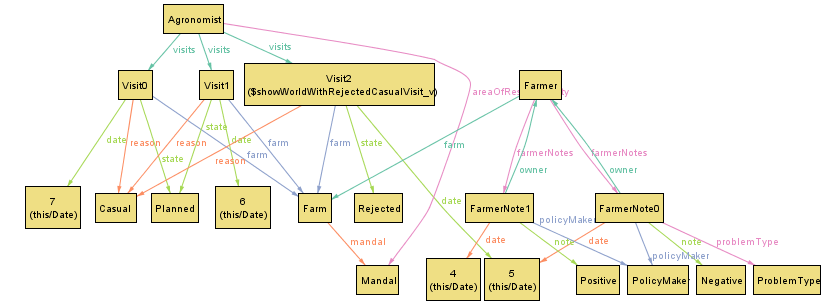
\includegraphics[width=\textwidth, keepaspectratio, origin=c]{alloy/world_instances/showWorldWithRejectedCasualVisit2.png}
    \caption{World instance focused on visits - rejected, causal visit}
    \label{fig:rejected_causal}
\end{figure}

 The first instance of worlds presented in Figure \ref{fig:rejected_causal} shows that as stated in \textbf{R63}, if a casual visit is rejected, then a new casual visit is planned.
 
\begin{figure}[H]
    \centering
    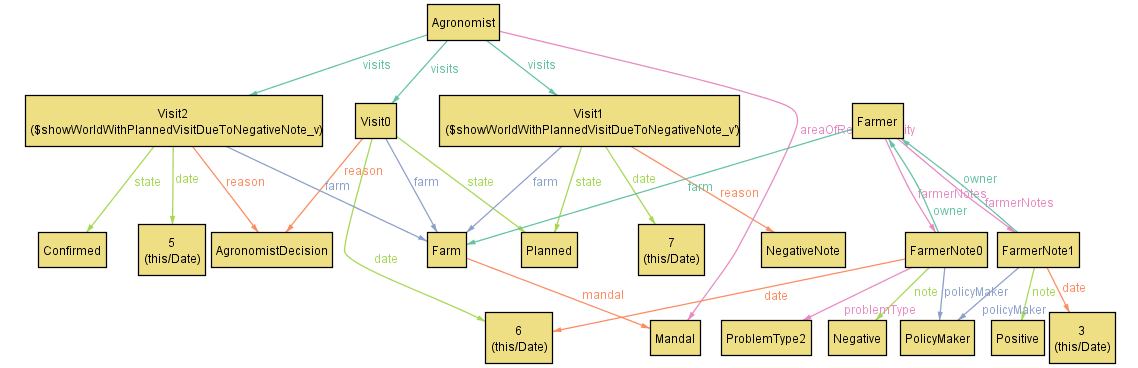
\includegraphics[width=\textwidth, keepaspectratio, origin=c]{alloy/world_instances/showWorldWithPlannedVisitDueToNegativeNote2.png}
    \caption{World instance focused on visits - planned, due to negative note visit}
    \label{fig:planned_negative_note}
\end{figure}

The world instance presented in figure \ref{fig:planned_negative_note} shows usage of the fact \textit{NoVisitDueToNegativeNoteIsPlannedBeforeTheDateOfTheLastNegativeNote} as the visit due to negative note is planned on \textit{date = 7} whilst the negative note was given on \textit{date = 6}. Another requirement (\textbf{R58}) fulfillment that can be noticed is that only a visit on or after the current day can be confirmed (it follows the state chart presented in figure \ref{fig:state_diagram}). The aforementioned requirement is exemplified with the date of the \textit{Visit2} (\textit{date = 5}, according to the alloy script in the previous section the \textit{currentDay = 5}).

\begin{figure}[H]
    \centering
    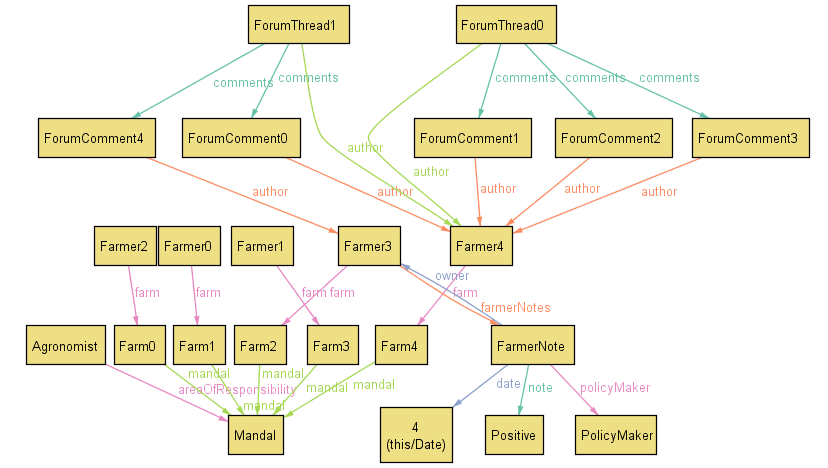
\includegraphics[width=\textwidth, keepaspectratio, origin=c]{alloy/world_instances/showWorldFocusedOnForum2.png}
    \caption{World instance focused on farmer's forum}
    \label{fig:forum}
\end{figure}

The third world instance (figure \ref{fig:forum}) shows many atoms related to farmer's forum. Two forum threads are created by two different farmers and some comments are added. In addition, as assumptions \textbf{A1} and \textbf{A5} state, each farmer possesses exactly one farm that belongs to exactly one mandal. 

\begin{figure}[H]
    \centering
    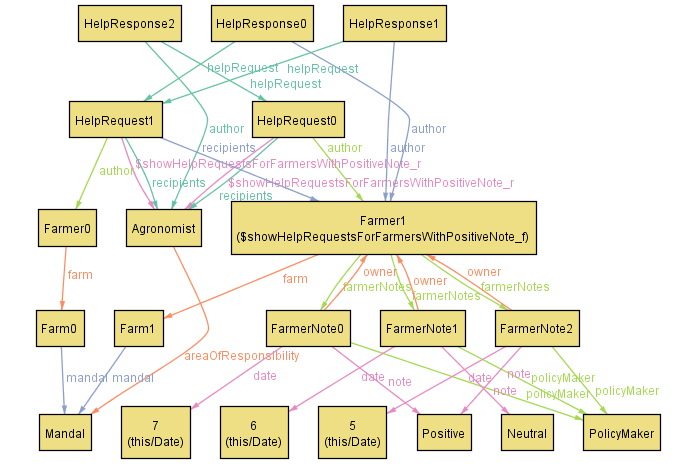
\includegraphics[width=\textwidth, keepaspectratio, origin=c]{alloy/world_instances/showHelpRequestsForFarmersWithPositiveNote2.png}
    \caption{World instance focused on help requests}
    \label{fig:help_requests}
\end{figure}
The fourth world instance (figure \ref{fig:help_requests}) focuses on help requests and responses. First, both help requests are obtained by an agronomist that takes care of the mandal (the mandal is inside the agronomist's area of responsibility) in which the author of the help request has his farm. Secondly, the \textit{Farmer1} who created help responses is a farmer with a positive note as, which matches the requirement \textbf{R35}.


\begin{figure}[H]
    \centering
    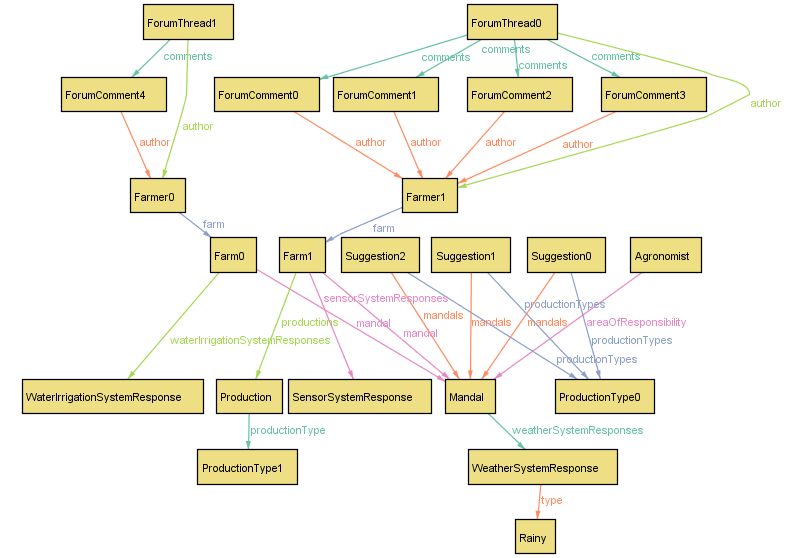
\includegraphics[width=\textwidth, keepaspectratio, origin=c]{alloy/world_instances/General2.png}
    \caption{World instance without visits (focus shifted to other atoms)}
    \label{fig:general_world}
\end{figure}

The last figure, figure \ref{fig:general_world}, presents an instance created with the least number of constraints. It contains some types that were not presented on previous figures for clarity. For instance, atoms presenting the production of \textit{Farm1} are depicted.